\documentclass[10pt]{article}
\usepackage[T1]{fontenc}
\usepackage[margin=0.9in]{geometry}
\usepackage{graphicx,booktabs,enumitem,amssymb,caption}
\usepackage[hidelinks]{hyperref}
\setlist{nosep,leftmargin=1.2em}
\emergencystretch=3em
\setlength{\parskip}{4pt}\setlength{\parindent}{0pt}

\title{CMSC614 Project M3: Figure and Experiment Log}
\author{Hojin Choi, Andrew Kim}

\begin{document}
{\centering{\large\bfseries CMSC614 Project M3: Figure and Experiment Log}\\[2pt]
Hojin Choi, Andrew Kim\\}
\vspace{6pt}


\noindent\begin{minipage}{\linewidth}
\centering
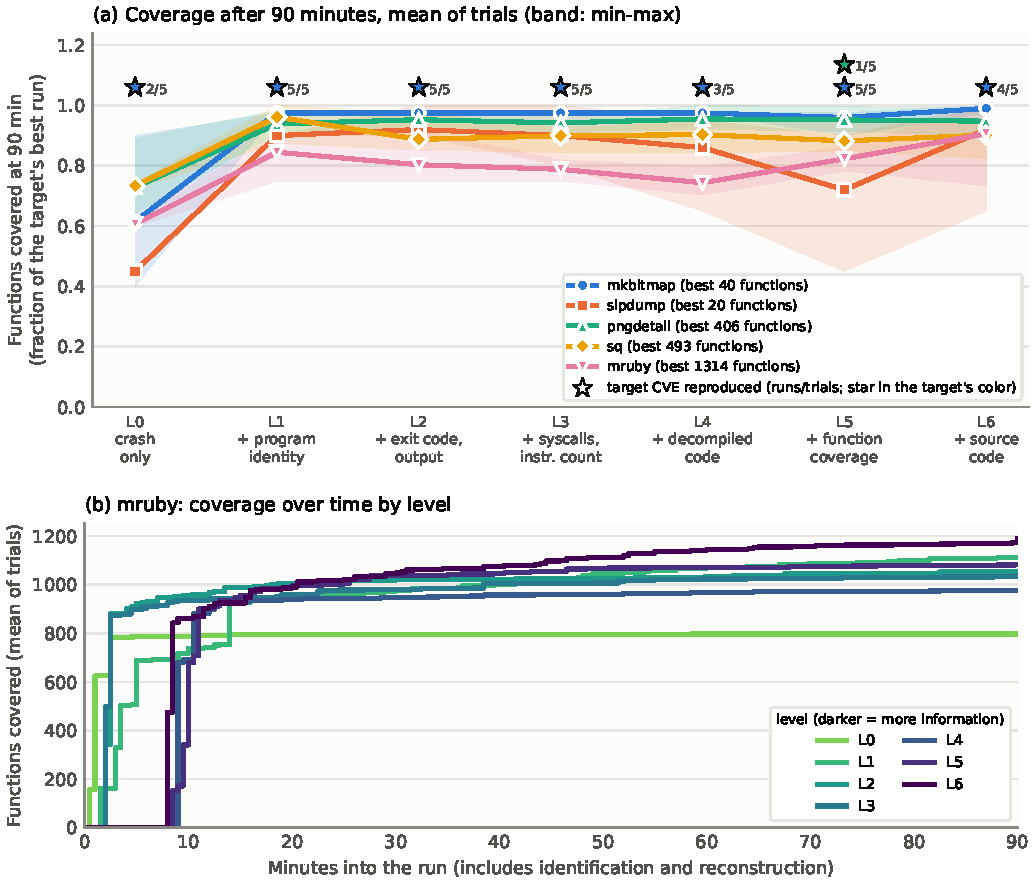
\includegraphics[width=\linewidth]{figure_time.pdf}
\small
\captionof{figure}{\textbf{Coverage and CVE reproduction as the LLM gets more information
(L0\(\to\)L6), 90 minutes per run.} Same engine and LLM (Qwen3.8-27B) at every level; each level
adds one kind of information, from crash/no crash (L0) up to source code (L6). 5 targets,
5 trials each. Coverage = distinct functions executed by a run's inputs, measured afterwards on
the debug build.
\textbf{(a)} Coverage at 90 min relative to the target's best run (line: mean, band: min--max).
Stars: target CVE reproduced, in \(n\) of 5 trials.
\textbf{(b)} mruby, our largest target, over time. L4--L6 start about 6 minutes later because
they first spend calls on reconstruction.
Going from L0 to L1 (telling the LLM what the program is) raises coverage on every target
(Mann--Whitney, \(p \le 0.006\)). Past L1 we see no reliable gain; on mruby L4 is even lower
(\(p = 0.04\), uncorrected).}
\label{fig:ladder}
\end{minipage}

\begin{table}[h]
\centering\scriptsize\setlength{\tabcolsep}{2.5pt}
\resizebox{\linewidth}{!}{\begin{tabular}{lccccccc}
\toprule
Target & L0 & L1 & L2 & L3 & L4 & L5 & L6 \\
\midrule
mkbitmap & 19 (16--36)$^{\star2}$ & 39 (39--39)$^{\star5}$ & 39 (39--39)$^{\star5}$ & 39 (39--39)$^{\star5}$ & 39 (39--39)$^{\star3}$ & 39 (36--39)$^{\star5}$ & 40 (39--40)$^{\star4}$ \\
sipdump & 9 (9--9) & 18 (18--18) & 18 (18--20) & 18 (16--20) & 18 (13--19) & 18 (9--18) & 20 (13--20) \\
pngdetail & 286 (261--362) & 381 (368--399) & 389 (376--396) & 384 (369--391) & 383 (374--406) & 384 (371--404)$^{\star1}$ & 387 (365--403) \\
sq & 360 (357--366) & 486 (431--493) & 424 (420--481) & 448 (416--456) & 445 (416--468) & 436 (418--465) & 448 (406--465) \\
mruby & 788 (786--825) & 1126 (984--1184) & 1041 (984--1205) & 1035 (984--1076) & 937 (925--1046) & 1102 (1029--1133) & 1249 (963--1314) \\
\midrule
LLM calls (mean) & 27.8 & 27.6 & 25.1 & 23.9 & 23.4 & 24.1 & 24.0 \\
\bottomrule
\end{tabular}
}
\caption{Numbers behind Figure~\ref{fig:ladder}: functions covered in 90 min, median
(min--max) over trials 2--6; \(\star n\) = CVE reproduced in \(n\) trials. Last row: mean LLM
calls in 90 min, similar across levels.}
\label{tab:data}
\end{table}

\section*{Experiment log}

Setup: 27-entry dataset (28 binaries, 31 PoCs) on the UMIACS Nexus cluster, inside an Ubuntu
24.04 Apptainer image because the nodes' glibc is too old for the binaries. LLM is Qwen3.8-27B
(FP8, vLLM, 2$\times$A5000). Each round the LLM writes a Python script that makes up to 8
inputs, we run them, and what we see goes into the next prompt. A run ``reproduces'' the CVE if
a crash matches the PoC's crash site on the debug build.

\subsection*{Nov 7}
\begin{itemize}
\item Went through the dataset. 27 entries, 28 binaries, 31 PoCs; everything from small tools
(mkbitmap, jhead) and binutils to media decoders and script interpreters (mruby, mujs, picoc).
\end{itemize}

\subsection*{Nov 13}
\begin{itemize}
\item Built the image, replayed all 31 PoCs: 30 crash. eu-strip (CVE-2025-1377) never does,
probably libelf 0.192 vs.\ 0.190 in our image. 5 READMEs had no run command, so we guessed;
4 of those crash where expected.
\item Smoke test on mkbitmap, 3 LLM calls, just to see the loop run end to end. Call 1: the LLM
identified the program and its formats (PNM/BMP) from \texttt{-{}-help} and strings alone.
Call 2: syntax error, no files. Call 3: an 11-byte PGM with zero width/height hit the CVE at
2.7 min, but the same script then tried to write a 16\,MB file and got killed. Added prompt
rules: one try/except per file, keep files under 1\,MB.
\item Picked 5 pilot targets with different input types and sizes: mkbitmap (images), sipdump
(pcap), pngdetail (PNG), sq (sq programs), mruby (Ruby). Kept them for everything after.
\item Pilot v1, 15 calls each: 0/5. Scripts mostly swallowed their own exceptions or did not
parse.
\item Pilot v2 (syntax check + one repair call, show stderr, ``try something different'' after
3 stale rounds): 1/5, mkbitmap. Repairs ate up to 7 of 15 calls --- turned out to be our bug,
Qwen leaves the code fence open and our extractor kept the fence line. pngdetail replies were
also getting cut at 4096 tokens.
\item Pilot v3: fixed both. Still 1/5, but now every round produces files.
\end{itemize}

\subsection*{Nov 14}
\begin{itemize}
\item Set up Ghidra for reconstruction. It ignored our heap setting until we found that 12.2
reads \texttt{GHIDRA\_HEADLESS\_MAXMEM} instead.
\item The dataset binaries print things like ``[*] HEAP BUFFER OVERFLOW Detected!'' from their
instrumentation. We hide those functions from the decompiled code so the LLM can't just read the
bug condition. First filter was too broad.
\item Pilot v4 with reconstruction: 1/5 (mkbitmap). Reconstruction costs 3--4 of the 15 calls.
\item Tried a white-box baseline adapted from WhiteFox (OOPSLA'24, originally for compilers).
v1: 1/10. sq crashed at setup (``::'' from a C++ name in a log file name), and the LLM wrote
JavaScript for sq. v2: 1/10 again, sq inputs still did not parse.
\item Ghidra export for all 28 binaries. sam2p and mujs-pp were fully stripped, so we rebuilt
them with symbols (forgot \texttt{-{}-enable-gif} the first time). All 28 ready.
\end{itemize}

\subsection*{Nov 15}
\begin{itemize}
\item Putting WhiteFox on hold; not clear yet how to make it a fair baseline.
\item Coverage tool: one-shot gdb breakpoint on every function, replay inputs on the debug
build. Missed weak C++ symbols at first (pngdetail 348 vs.\ 962 functions).
\item Ladder smoke test: L0 found the mkbitmap bug in one call, which should not happen. Our
prompt's example file name was \texttt{03\_large\_width.bmp} --- basically a hint. Removed it.
All earlier mkbitmap results are biased by this.
\item First ladder pilot used a call budget (15 calls, stop at first hit). Runs took 8--41 min
and L4--L6 lose calls to reconstruction, so it wasn't fair. Switched to a 90-minute wall-clock
budget and no early stop.
\item Wanted to run trials in parallel but we were at the GPU limit, so one server, 35 runs at
a time, trials back to back.
\item Trial 1: sq L1/L2 lost ${\sim}$40 min each to our fixed 600\,s LLM timeout plus retry.
Fixed (waits now end at the run's deadline). Trial 1 is left out of the figure.
\item mruby coverage measurement got OOM-killed twice; one generated script allocates forever.
Capped gdb at 6\,GB.
\item Trials 2 and 3: clean. Runs can overrun by a reply (up to 2.5 min), so we cut everything
at exactly 90 min.
\end{itemize}

\subsection*{Nov 16}
\begin{itemize}
\item Two trials aren't enough to say anything past L1, so we ran trials 4--6, same code, one
LLM server each, in parallel. No errors.
\item pngdetail's CVE reproduced for the first time (L5, trial 5, 61 min). mkbitmap also hit at
L0 twice. Checked the L0 prompt again, nothing leaks (it only shows \texttt{./target @@}), so
the LLM just guessed BMP.
\item Redid the figure and table with trials 2--6 and ran Mann--Whitney per target. L1 > L0
everywhere. Past L1 nothing holds up; mruby L6 looked best with 2 trials but not with 5
(\(p = 0.42\)). No multiple-comparison correction.
\end{itemize}

\subsection*{Limitations}
\begin{itemize}
\item 5 trials, 5 of 28 targets, 90 min per run (fuzzing papers usually do 24\,h).
\item Runs share an LLM server, so equal time $\approx$ equal calls (23--28) only under this load.
\item mkbitmap's bug is easy, so it's a sanity check. Of the other four, only pngdetail was hit
in trials 2--6 (once).
\item Qwen may already know these programs and CVEs.
\item Function coverage is coarser than edge coverage.
\end{itemize}

\end{document}
